\documentclass[a4paper,11pt]{article}
\usepackage{geometry}
 \geometry{
 a4paper,
 total={170mm,257mm},
 left=20mm,
 top=20mm,
 }


 \usepackage{amsmath}
 \usepackage{siunitx}
 \usepackage{multirow}
\usepackage{colortbl}
 \usepackage{hhline}

 \usepackage{lipsum}  %%% Lorem ipsum

\setlength{\headheight}{30.0pt}
\setlength{\footskip}{20pt}


\usepackage{hyperref}
\hypersetup{
    colorlinks=True,
    linkcolor={blue!20!black},
    filecolor=magenta,      
    urlcolor=cyan,
}



 \usepackage[export]{adjustbox}
\usepackage[english]{babel}
\usepackage[utf8]{inputenc}
\usepackage{fancyhdr}
\usepackage{multicol}

\pagestyle{fancy}
\fancyhf{}
\rhead{\textit{Pul074BEX004}}
\lhead{\textit{Amrit Prasad Phuyal}}
\rfoot{\thepage}


\usepackage{mathpazo} % Palatino font
\usepackage{graphicx}
\usepackage{float}


%%%%%% include  Titles.%%%% use \input{./CP}%%%
%%%use """"""""    \CP{}{}{}{}   """" %%%% and 4 argument to craete Title page 
%%%%%%%%%%%%%%%%%%%%%%%%%%%%%%%%%%%%%%%%%%%%%%%%%%%%%%%%%%%%%%%%%
%%%argument number
%% 1=major header ## Course name 
%% 2=minor4 heading ## lab/assignmet no
%% 3=Title  ## Assignment or Lab title
%% 4=submitted to::## input receiver Name"
%%%%%%%%%%%%%%%%%%%%%%%%%%%%%%%%%%%%%%%%%%%%%%%%%%%%%%%%%%%%%%%%%


\usepackage{mathpazo} % Palatino font
\usepackage{graphicx}
\usepackage{float}

%%% format and command for lab ans c and assembly

\newcommand{\HRule}{\rule{\linewidth}{0.4mm}} % Defines a new command for horizontal lines, change thickness here



%----------------------------------------------------------------------------------------
%	TITLE PAGE
%----------------------------------------------------------------------------------------


\newcommand{\CP}[4]{ \begin{titlepage} % Suppresses displaying the page number on the title page and the subsequent page counts as page 1
		%%%%  univerdity logo%%
		\begin{figure}[H]
			\centering
			
\includegraphics[scale=0.13]{tulogo.jpg}
		\end{figure}
		%%% end university logo

		\center % Centre everything on the page

		%------------------------------------------------
		%	Headings
		%------------------------------------------------

		\textsc{\huge Institute of Engineering \\ Central Campus,Pulchowk}\\[1.5cm] % Main heading such as the name of your university/college

		\textsc{\Large #1}\\[0.5cm] % Major heading such as course name

		\textsc{\large #2}\\[0.5cm] % Minor heading such as assignment no./ lab no.

		%------------------------------------------------
		%	Title
		%------------------------------------------------

		\HRule\\[0.4cm]

		{\Huge\bfseries #3}\\[0.4cm] % Title of your document

		\HRule\\[1.5cm]

		%------------------------------------------------
		%	Author(s)
		%------------------------------------------------
		\vfill\vfill
		\begin{minipage}{0.4\textwidth}
			\begin{flushleft}
				\large{
				\textbf{Submitted BY:}\\
				{\normalsize AMRIT PRASAD PHUYAL}\\ % NAME
				{\normalsize Roll: PULL074BEX004}} % Roll
			\end{flushleft}
		\end{minipage}
		~
		\begin{minipage}{0.4\textwidth}
			\begin{flushright}
				\large
				\textbf{Submitted To:}\\
				{ \normalsize{#4}\\ }% recepent's  Name 
				{\normalsize Department of Electronics and Computer Engineering}
			\end{flushright}
		\end{minipage}

		%------------------------------------------------
		%	Date
		%------------------------------------------------

		\vfill\vfill\vfill % Position the date 3/4 down the remaining page

		{\large\today} % Date, change the \today to a set date if you want to be precise

		\vfill % Push the date up 1/4 of the remaining page

	\end{titlepage}
} %%% cover page

%%% Formating And Command for Embedded Lab  VHDl
%% \ancode{caption}{Filename}


\usepackage{listings}
\usepackage{multicol}
\usepackage{mdframed}

\renewcommand{\lstlistlistingname}{List of MATLAB Codes}
\renewcommand{\lstlistingname}{MATLAB Code}

\setlength{\columnsep}{0.5cm}

\usepackage{xcolor}
\definecolor{codegreen}{rgb}{0,0.6,0}
\definecolor{codegray}{rgb}{0.3,0.3,0.3}
\definecolor{codepurple}{rgb}{0.58,0,0.82}
%\definecolor{backcolour}{rgb}{0.95,0.99,0.92}
\definecolor{backcolour}{rgb}{0,0,0}

\lstdefinestyle{MATLAB}{
  %backgroundcolor=\color{backcolour},  
  commentstyle=\color{codegreen},
  keywordstyle=\color{blue},
  numberstyle=\tiny\color{codegray},
  stringstyle=\color{codepurple},
  basicstyle=\ttfamily\small\color{black},
  breakatwhitespace=false,
  breaklines=true,
  captionpos=b,
  keepspaces=true,
  language=Matlab,
  numbers=left,
  numbersep=5pt,
  showspaces=false,
  frame = single,
  showstringspaces=false,
  showtabs=false,
  tabsize=3
}




\newcommand {\anscode}[2]{
  \lstinputlisting[style=MATLAB,nolol]{#2}

  \begingroup
  \captionof{lstlisting}{#1}
  \endgroup

}

%%% Formating And Command for Embedded Lab  VHDL %%% Matlab code



%%%%%%%%%%%%%%%%%%%%%% for matlab observation #1 fig name #2 Caption
\newcommand{\mobs}[2]{
    \begin{figure}[H]
        \centering
        \includegraphics[width=0.9\linewidth]{./FIG/#1.eps}
        \caption{#2}
    \end{figure}
   
}







\begin{document}


%%%%  COver page 
\CP{Communication System II}{Lab \#1}{Amplitude Modulation \& Demodulation}
{Suman Sharma}
%%%%%%%%%%%%%%%%%%%%

\pagenumbering{gobble}
\renewcommand{\contentsname}{Table of Contents}
\tableofcontents

% \pagebreak
%\listoffigures
\pagebreak
% \listoftables
% \vspace{5em}
\lstlistoflistings
%\pagebreak
\vspace{10em}
\listoffigures
\pagebreak
\pagenumbering{arabic}

%%%%%%%%%%%%%%%%%%%%%%%%%%%%%%%%%%%%%%%%%%%%%%
\section{Title} {\large Amplitude Modulation \& Demodulation}
%%%%%%%%%%%%%%%%%%%%%%%%%%%%
\section{Objective}
\begin{itemize}
    \item To view amplitude modulation for DSB­-TC, DSB­-SC, SSB  and Amplitude demodulation.

\end{itemize}
%%%%%%%%%%%%%%%%%%%%%

\section{Theory}
\subsection{Amplitude modulaton}
If amplitude of carrier wave varies in accordance with the amplitude of the signal, then the signal is called amplitude modulation.
\begin{figure}[H]
    \centering
    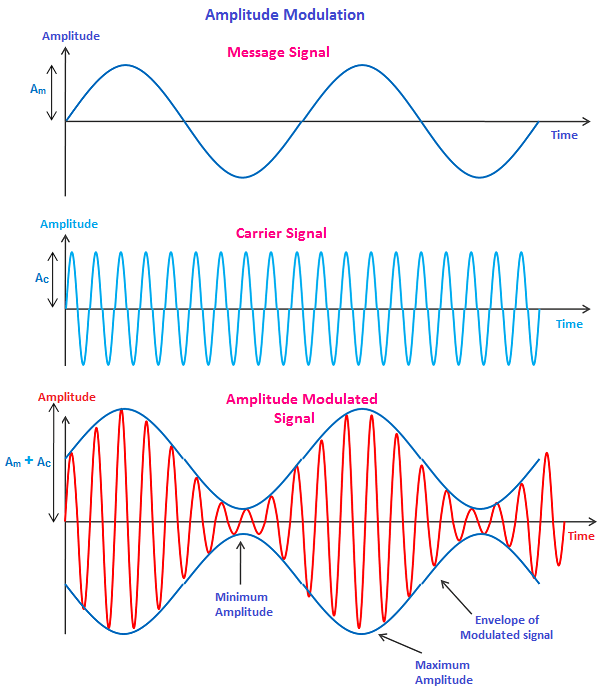
\includegraphics[width=0.85\linewidth]{./FIG/amplmod.png}
    \caption{Amplitude modulation}
\end{figure}

\subsubsection{DSB-­TC}
Double Sideband Transmitted carrier (DSB-TC) is a type of amplitude modulation where modulated signal has full carrier representation.For DSB-FC modulated signal $y(t)$ of a message signal $m(t)$ having carrier signal of frequency $f_c$ :

\begin{equation}
    y(t) = (1 + \mu m(t))cos(2\pi f_c t)
\end{equation}
where, $\mu$ is the \textbf{modulation index}.
\begin{itemize}
    \centering
    \item $\mu < 1$: Under modulation
    \item $\mu = 1$: Perfect modulation
    \item $\mu > 1$: Over modulation
\end{itemize}


\subsubsection{DSB­-SC}
Double Sideband-Suppressed Carrier (DSB-SC) is a type of amplitude modulation where modulated signal has reduced carrier representation in order to save power. For DSB-SC modulated signal $y(t)$ of a message signal $m(t)$ having carrier signal of frequency $f_c$ :


\begin{equation}
    y(t) = A_c m(t)cos(2\pi f_c t)
\end{equation}

\subsubsection{SSB}
Single Sideband is a type of amplitude modulation where modulated signal has reduced carrier representation in order to save power and additionally Suppressing one of the side band.. For SSB modulated signal $y(t)$ of a message signal $m(t)$ having carrier signal of frequency $f_c$ :


\begin{equation}
    y(t) = m(t)cos(2\pi f_c t) - \hat{m}(t)sin(2\pi f_c t)
\end{equation}
where $\hat{m}(t)$ is the \textbf{Hilbert transform} of the message signal.

\subsection{Amplitude Demodulation}
Amplitude Demodulation is the process of demodulating the received signal to recover the original message.

\section{Problems}
%%%%%%%%111111111111111111111111
\subsection{DSB-TC(Under,Normal,Over)}

\MAT{./CODES/amdsbtc.m}{MATLAB code DSB-TC}
\mobs{dsbtc}{DSB-TC(Under,Normal,Over)}


%%%%%%%%%%%%%%%%%%%%%%%%22222222222222222222222222
\subsection{DSB-SC (Time \& Frequency Domain)}
\MAT{./CODES/amdsbsc.m}{MATLAB code DSB-SC}
\mobs{dsbsc}{DSB-SC (Time \& Frequency Domain)}


\pagebreak
%%%%%%%%%%%%%%%%%%%33333333333333333333333333
\subsection{SSB (Time \& Frequency Domain)}

\MAT{./CODES/amssb.m}{MATLAB code SSB}
\mobs{ssb}{SSB (Time \& Frequency Domain)}
%%%%%%%%%%%%%%%%%%%44444444444444444444444

\pagebreak
\subsection{Demodulation}
\MAT{./CODES/demodulation.m}{MATLAB code Demodulation}
\mobs{demod}{Demodulation Observation of DSB-SC}

\section{Discussion and Conclusion}
In this lab we observed amplitude modulation of DSB-TC, DSB-SC, SSB and Demodulation of DSB-SC signal.We used MATLAB an its modules to implement the above mentioned process and generating plots.

\end{document}